\newcounter{reqCounter} % Define a custom counter for functional requirements
\stepcounter{reqCounter}

\newcounter{ucCounter} % Define a custom counter for functional requirements
\stepcounter{ucCounter}


Within this section can be found a list of functional requirements for S\&C, categorized by the major features of the platform.

\paragraph{Registration of Students}
\begin{itemize}[label={[\textbf{FR\arabic{reqCounter}}]}, align=left, leftmargin=*]
    \item \stepcounter{reqCounter} The system shall allow new student users to register on the platform using their respective institutional accounts.
    \item \stepcounter{reqCounter} After an institutional account has been linked with the platform, the system shall allow student users to log in using their institutional credentials.
    \item \stepcounter{reqCounter} The system shall allow the registration of student users only if they are classified as students within the institutional account they provide.
\end{itemize}

\paragraph{Registration of Companies}
\begin{itemize}[label={[\textbf{FR\arabic{reqCounter}}]}, align=left, leftmargin=*]
    \item \stepcounter{reqCounter} The system shall allow new company users to register on the platform using a valid email address.
    \item \stepcounter{reqCounter} After providing an email address, the system shall verify the provided address through a verification email.
    \item \stepcounter{reqCounter} After the new company user has verified their email, the system shall generate and deliver a password for the newly created account via the verified email.
    \item \stepcounter{reqCounter} The system shall allow the company user to log in using the validated email address and the provided password.
    \item \stepcounter{reqCounter} Upon the first login, the system shall require the new user to provide a certificate from the relevant tax authority, including the company name and unique identifier. The system shall also require the full company name and unique identifier to be entered manually in the relevant input fields alongside the certificate.
    \item \stepcounter{reqCounter} The system shall retain company user data only at two points: first, after successful email verification, where the provided email address and generated password will be retained as login credentials; and second, after submitting the initial verification information, where all submitted data up to that point shall be retained.
\end{itemize}



\paragraph{Registration of Universities}
\begin{itemize}[label={[\textbf{FR\arabic{reqCounter}}]}, align=left, leftmargin=*]
    \item \stepcounter{reqCounter} The system shall allow new university users to register on the platform using pre-designated institutional accounts allocated for S\&C.
    \item \stepcounter{reqCounter} After an institutional account has been linked with the platform, the system shall allow university users to log in using their institutional credentials.
    \item \stepcounter{reqCounter} If the institutional account has not been pre-designated for use on S\&C, the system shall reject the registration attempt.
\end{itemize}

\paragraph{Profile Management}
\begin{itemize}[label={[\textbf{FR\arabic{reqCounter}}]}, align=left, leftmargin=*]
    \item \stepcounter{reqCounter} The system shall, by default, provide a blank profile template for all users.
    \item \stepcounter{reqCounter} The system shall provide different collections of predetermined fields based on the user type.
    \item \stepcounter{reqCounter} The system shall allow all users to edit each field in their profile, with the exception of unique identifiers, such as tax numbers for companies and universities, and unique IDs for students, which cannot be altered.
    \item \stepcounter{reqCounter} The system shall allow each field to be configured as public or private, provided that data is present in the respective field.
    \item \stepcounter{reqCounter} The system shall automatically configure all fields with no data as private.
    \item \stepcounter{reqCounter} The system shall allow all users to provide public hyperlinks to other platforms which the system shall display in a format that clearly indicates the platform to which the hyperlink leads to.
    \item \stepcounter{reqCounter} The system shall integrate OpenAI's ChatGPT 4.0 API into each field to provide AI-generated suggestions for profile improvements.
\end{itemize}



\paragraph{Internship Advertisement Creation and Management}
\begin{itemize}[label={[\textbf{FR\arabic{reqCounter}}]}, align=left, leftmargin=*]
    \item \stepcounter{reqCounter} The system shall only allow company users whose data has been verified to create, update, and delete public internship advertisements, where the system shall save unfinished advertisements as draft.
    \item \stepcounter{reqCounter} The system shall allow the creation of new internship advertisements only if they possess the following fields: name, internship duration, short description, location, internship type, and the number of stages in the application process.
    \item \stepcounter{reqCounter} The system shall integrate OpenAI's ChatGPT 4.0 API into each field of the internship advertisement creation process to provide AI-generated suggestions for enhancing the advertisement.
    \item \stepcounter{reqCounter} The system shall allow for numerous types of stages to be created, including but not limited to questionnaires and video interviews, which may be scheduled on external platforms.
   
    \item \stepcounter{reqCounter} Should the internship creation process be interrupted at any stage, the system shall save the unfinished internship advertisement as a draft.
    \item \stepcounter{reqCounter} After creation, the system shall allow company users to make updates to all fields of each internship advertisement they have created, with the exception of that internship advertisement's unique ID and publication timestamp.
\end{itemize}

\paragraph{Internship Search, Application, and Management of Applications}
\begin{itemize}[label={[\textbf{FR\arabic{reqCounter}}]}, align=left, leftmargin=*]
    \item \stepcounter{reqCounter} The system shall analyze the profile of the student user upon login and recommend 3 internship advertisements based on matching qualifications and background, and display these recommendations prominently to the student user.
    \item \stepcounter{reqCounter} The system shall allow student and university users to view all internship advertisements posted by any company on the platform, not just those they are applying to. Company users, however, will only be allowed to view and manage the advertisements they have created.
    \item \stepcounter{reqCounter} The system shall allow all student users to apply to internship advertisements, after which their profiles will be automatically inserted into the list of applicants under the Stage 1 category.
    \item \stepcounter{reqCounter} Upon a successfully submitted application, the system shall notify the advertisement's creator.
    \item \stepcounter{reqCounter} The system shall only allow company users who are creators of the internship advertisement to move candidates further along the selection stages.
    \item \stepcounter{reqCounter} The system shall allow the company user, at any given stage, to reject any candidate without mandating a reason.
    \item \stepcounter{reqCounter} Upon a change in status, be it a rejection or a move up in the selection stages, the system shall always notify the candidate of the change.
    \item \stepcounter{reqCounter} Upon reaching the final stage as designated by the company, the system shall automatically classify the candidate as accepted for the internship.
    \item \stepcounter{reqCounter} The system shall allow the company user to request the commencement of an internship from the candidate's host university. After the internship is approved by the host university, it shall commence on a predetermined date.
\end{itemize}

\paragraph{Internship Monitoring, Complaint Management \& Feedback System}
\begin{itemize}[label={[\textbf{FR\arabic{reqCounter}}]}, align=left, leftmargin=*]
    \item \stepcounter{reqCounter} During any stage of the internship, the system shall allow both the candidate and the company user to submit a complaint to the host university, after which the university user shall be automatically notified.
    \item \stepcounter{reqCounter} After a complaint is received, the university may choose to resolve the complaint or to terminate the internship. The system shall allow for both choices to be submitted.
    \item \stepcounter{reqCounter} The system shall not allow the termination of an internship by any party except the university user. The system shall allow a termination only after a complaint has been submitted.
    \item \stepcounter{reqCounter} Upon the successful completion of an internship, the system shall request feedback from both the company user and the intern regarding the internship experience. Moreover, the system shall request feedback from all three users types involved in the internship regarding their satisfaction with S\&C.
    \item \stepcounter{reqCounter} The system shall request the university to review the submitted internship feedback. After the review, the system shall allow the university to either include the ratings in the profiles of both the student user and the company user, or keep the feedback private.
\end{itemize}


\subsubsection{Use cases Diagram}
\begin{figure}[H]
    \centering
    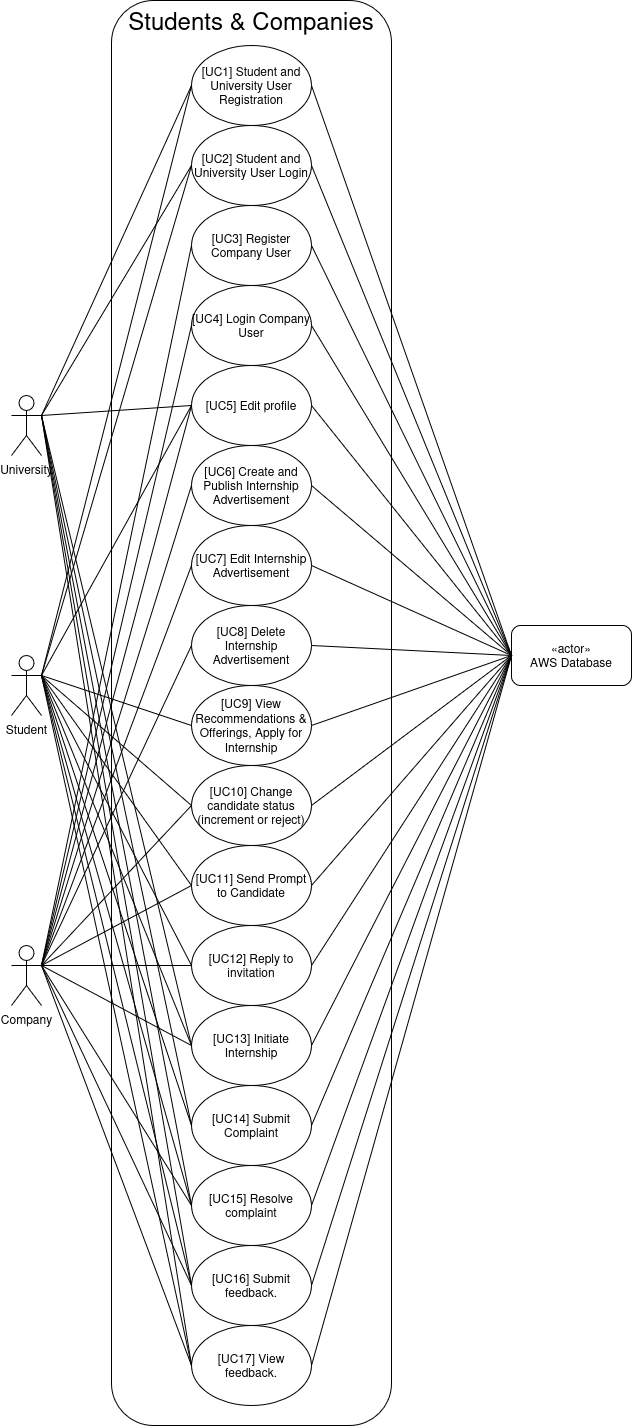
\includegraphics[height=0.9\textheight]{Diagram 4.png}
    \caption{Enter Caption}
    \label{fig:enter-label}
\end{figure}

\subsubsection{Use cases}
The following section presents the identified use cases for S\&C, using the fully dressed format.

\paragraph{Registration, Login \& Profile Editing}

\begin{itemize}[label={[\textbf{UC\arabic{ucCounter}}]}, align=left, leftmargin=*]
     \item \stepcounter{ucCounter} Student and University User Registration\\
     \textbf{Actors:} Student or University users\\
     \textbf{Preconditions:} The user has accessed the platform sign in page. The user has a institutionally provided account.\\
     \textbf{Success Guarantee (Postconditions):} The user is successfully registered on the platform.\\
     \textbf{Main Success Scenario (or Basic Flow):} 
     \begin{enumerate}[label=\arabic*.] 
        \item The enters their institutional email in the designated field.
        \item The user presses the 'Connect my university' button.
        \item The platform redirects the user to their institutional login page.
        \item The user successfully signs in using their institutional credentials.
        \item The user agrees to cross-platform data sharing and the terms of service.
        \item The platform redirects the user to the platform landing page.
     \end{enumerate} \\

    \textbf{Extensions (or Alternative Flows):} 
    \begin{enumerate}[label=\arabic*.]
        \item[*a.] At any point, the user disconnects or the system fails:
            \begin{enumerate}[label=\arabic*.]
                \item The user reconnects to the platform.
                    \begin{enumerate}[label=\alph*.]
                        \item[1a.] The platform fails to recover, or the user is unable to reconnect.
                    \end{enumerate}
                 \item The user begins the registration process from the beginning, unless fully registered already.
            \end{enumerate}
        \item[3a.] The user entered a badly formatted email:
            \begin{enumerate}[label=\arabic*.]
                \item The platform informs the user that the entered email invalid.
                \item The user re-enters his email resumes the registration process.
            \end{enumerate}
        \item[3b.] The user entered an email which is not connect to an institutional account, the platform is unable to redirect:
            \begin{enumerate}[label=\arabic*.]
                \item The platform informs the user that the entered email is not connected to an institutional account.
                \item The user re-enters his email and resumes the registration process.
            \end{enumerate}
        \item[3c.] The University user entered an email which is not pre-authorized for university user account creation.
        \item[3-6*.] The institution's login system goes offline. The user is unable to resume registration.
        \item[4a.] The user is unable to log in into his institutional account.
        \item[5a.] The user declines cross platform data sharing and terms of service.
        \item[6-7a.] The platform is unable to redirect the user.
    \end{enumerate}

    \begin{figure}[H]
    	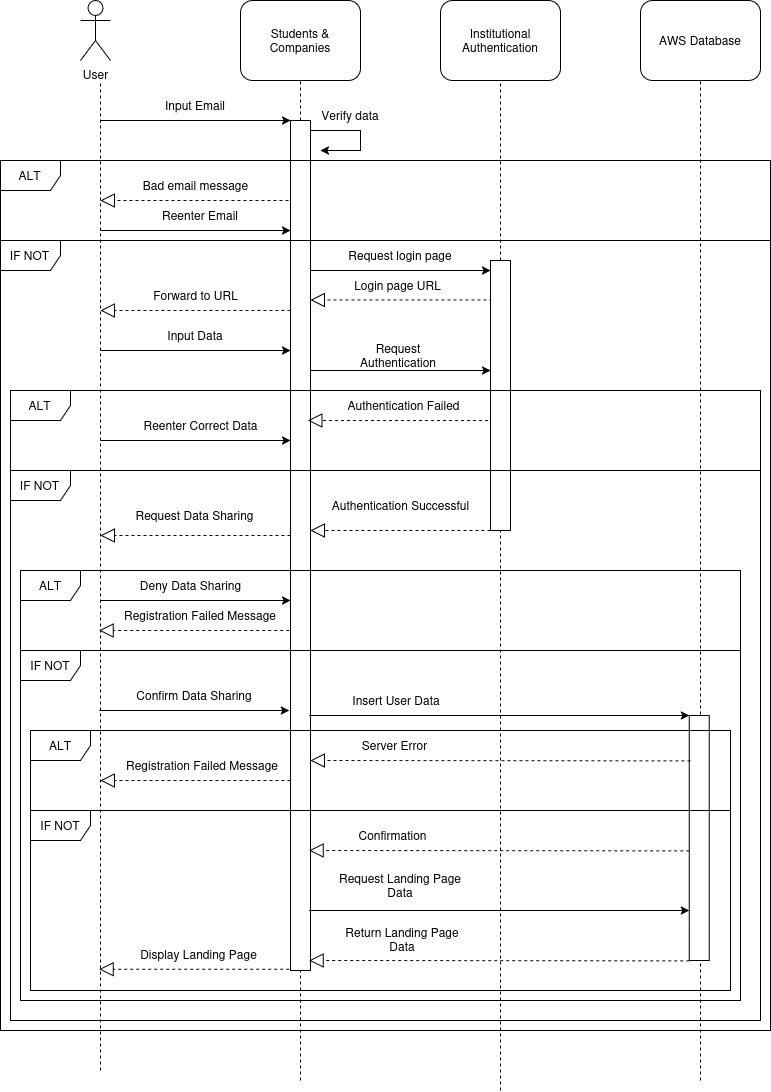
\includegraphics[width=\textwidth,height=\textheight,keepaspectratio]{RASD-Latex/assets/Use Case Diagrams/UC1.png}
    	\caption{UC1 - diagram}
    	\label{fig:DataRequest}
    \end{figure}

\newpage
    \item \stepcounter{ucCounter} Student and University User Login\\
     \textbf{Actors:} Student or University users\\
     \textbf{Preconditions:} The user has accessed the platform sign in page. The user has a institutionally provided account which is registered on the platform.\\
     \textbf{Success Guarantee (Postconditions):} The user is successfully logged in the platform.\\
     \textbf{Main Success Scenario (or Basic Flow):} 
     \begin{enumerate}[label=\arabic*.] 
        \item The user enters their institutional email in the designated field.
        \item The user presses the 'Connect my university' button.
        \item The platform redirects the user to their institutional login page.
        \item The user successfully signs in using their institutional credentials.
        \item The platform redirects the user to the platform landing page.
     \end{enumerate} \\

    \textbf{Extensions (or Alternative Flows):} 
    \begin{enumerate}[label=\arabic*.]
        \item[*a.] At any point, the user disconnects or the system fails:
            \begin{enumerate}[label=\arabic*.]
                \item The user reconnects to the platform.
                    \begin{enumerate}[label=\alph*.]
                        \item[1a.] The platform fails to recover, or the user is unable to reconnect.
                    \end{enumerate}
                 \item The user begins the login process from the beginning, unless already logged in.
            \end{enumerate}
        \item[3a.] The user entered a badly formatted email:
            \begin{enumerate}[label=\arabic*.]
                \item The platform informs the user that the entered email invalid.
                \item The user re-enters his email resumes the registration process.
            \end{enumerate}
        \item[3b.] The user entered an email which is not connect to an institutional account, the platform is unable to redirect:
            \begin{enumerate}[label=\arabic*.]
                \item The platform informs the user that the entered email is not connected to an institutional account.
                \item The user re-enters his email and resumes the registration process.
            \end{enumerate}
        \item[3-5*.] The institution's login system goes offline. The user is unable to resume the login process.
        \item[4a.] The user is unable to sign in into his institutional account.
        \item[4-5a.] The platform is unable to redirect the user.
        \end{enumerate}

    \begin{figure}[H]
    	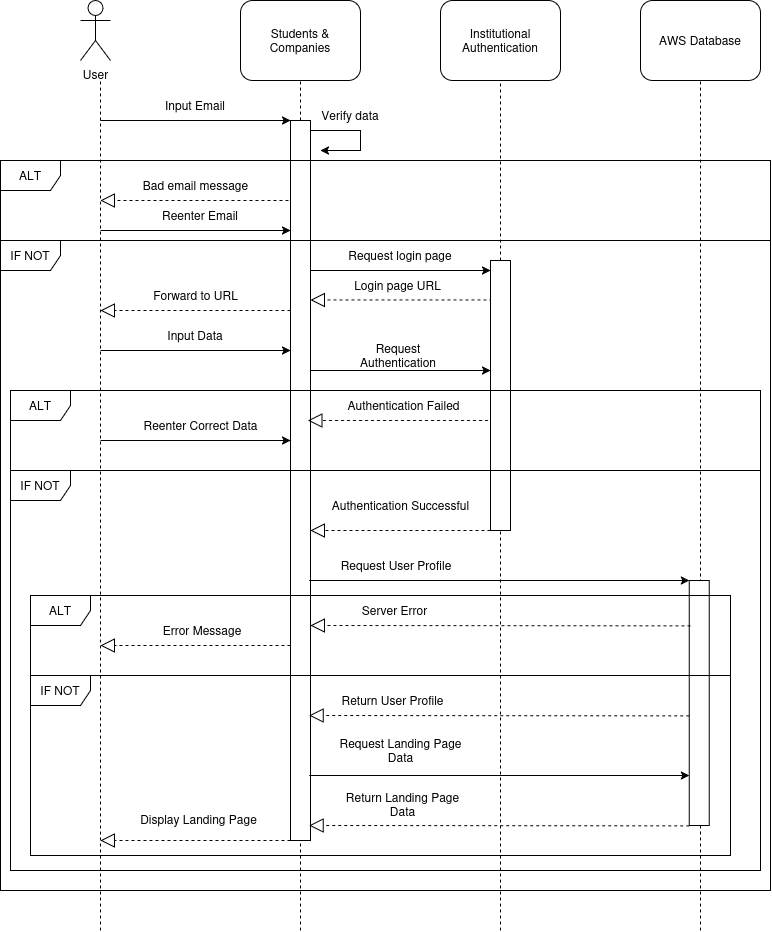
\includegraphics[width=\textwidth,height=\textheight,keepaspectratio]{RASD-Latex/assets/Use Case Diagrams/UC2.png}
    	\caption{UC2 - diagram}
    	\label{fig:DataRequest}
    \end{figure}
     
     
     \item \stepcounter{ucCounter} Register Company User \\
     \textbf{Actors:} Company user\\
     \textbf{Preconditions:} The company user has accessed the platform and is on the designated company sign up page. The company user has a valid email address to which they have access to. The company user possesses company tax identification documentation.\\
     \textbf{Success Guarantee (Postconditions):} The company user is successfully registered on the platform.\\
     \textbf{Main Success Scenario (or Basic Flow):} 
     \begin{enumerate}[label=\arabic*.] 
        \item The company user enters their desired email into the email field.
        \item The company user presses the 'Sign up' button.
        \item The platform sends a verification email and informs the user.
        \item The user receives the verification link and a password in the email.
        \item The user presses the verification link.
        \item The link redirects the user back to the platform. 
        \item The user is informed that their email has been verified.
        \item The user inputs the provided credentials, and successfully enters account creation.
        \item The user successfully uploads the company name, tax id and required tax certificate, and presses 'Submit'.
        \item The company user is redirected to the landing page of the platform.
     \end{enumerate} \\

    \textbf{Extensions (or Alternative Flows):} 
    \begin{enumerate}[label=\arabic*.]
        \item[*a.] At any point, the user disconnects or the system fails:
            \begin{enumerate}[label=\arabic*.]
                \item The user reconnects to the platform.
                    \begin{enumerate}[label=\alph*.]
                        \item[1a.] The platform fails to recover, or the user is unable to reconnect.
                    \end{enumerate}
                 \item The company user resumes the registration process from the last saved checkpoint.
            \end{enumerate}
        \item[1a.; 8a.] The user entered a badly formatted email.
            \begin{enumerate}[label=\arabic*.]
                \item The platform informs the user that the entered email invalid.
                \item The user re-enters his email resumes the registration process.
            \end{enumerate}
        \item[1b.] The entered email has already been resisted on the platform.
        \item[4a.] The user never receives the verification email.
        \item[5a.] The verification provided link fails to redirect.
            \begin{enumerate}[label=\arabic*.]
                \item The user copy-pastes the alternate link provided.
                    \begin{enumerate}[label=\alph*.]
                        \item[1a.] The alternative link is invalid. The user is unable to continue registration.
                    \end{enumerate}
                \item The user returns to the website and resumes the registration process.
            \end{enumerate}
        \item[8a.] The user's credentials are invalid.
        \item[9a.] The user is unable to upload his tax certificate.
    \end{enumerate}

     \begin{figure}[H]
    	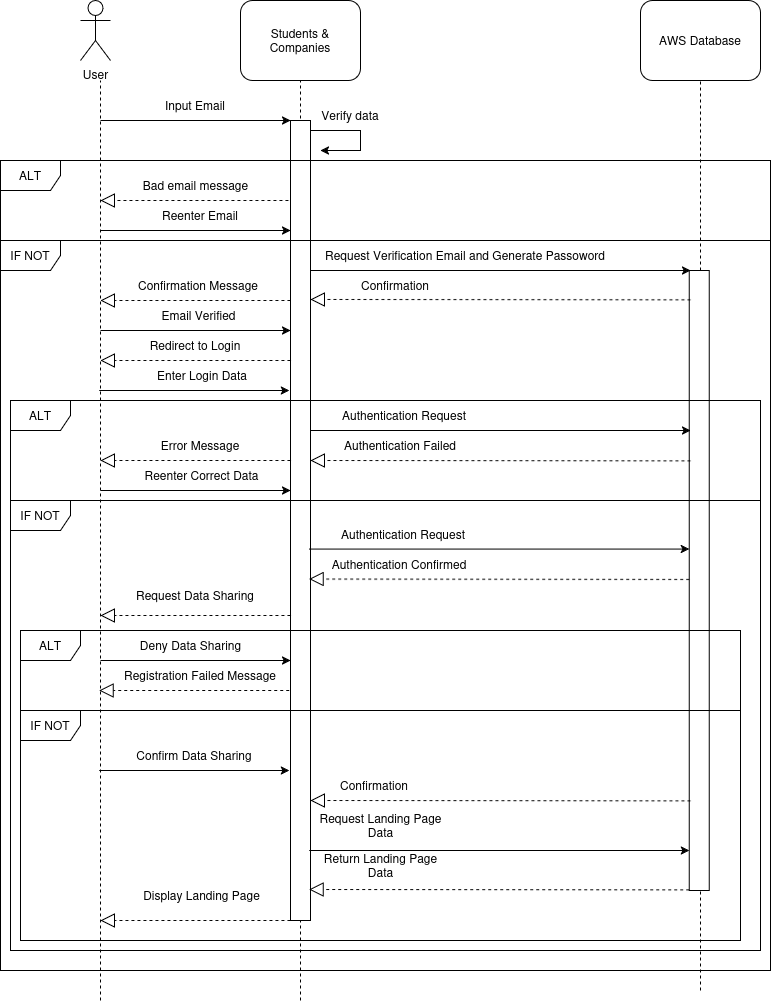
\includegraphics[width=\textwidth,height=\textheight,keepaspectratio]{RASD-Latex/assets/Use Case Diagrams/UC3.png}
    	\caption{UC3 - diagram}
    	\label{fig:DataRequest}
    \end{figure}
     
     \item \stepcounter{ucCounter} Login Company User \\
     \textbf{Actors:} Company User\\
     \textbf{Preconditions:} The company user has accessed the platform company login page. The company user is registered on the platform.\\
     \textbf{Success Guarantee (Postconditions):} The company user successfully logs in. \\
     \textbf{Main Success Scenario (or Basic Flow):} 
     \begin{enumerate}[label=\arabic*.] 
        \item The company user enters their credentials in the designated fields and presses the 'Log in' button.
        \item The user successfully signs in and the platform redirects the company user to the landing page.
     \end{enumerate} \\

    \textbf{Extensions (or Alternative Flows):} 
    \begin{enumerate}[label=\arabic*.]
        \item[*a.] At any point, the user disconnects or the system fails:
            \begin{enumerate}[label=\arabic*.]
                \item The user reconnects to the platform.
                    \begin{enumerate}[label=\alph*.]
                        \item[1a.] The platform fails to recover, or the user is unable to reconnect.
                    \end{enumerate}
                 \item The user begins the log in process from the beginning, unless already logged in.
            \end{enumerate}
        \item[1a.] The user entered a badly formatted email:
            \begin{enumerate}[label=\arabic*.]
                \item The platform informs the user that the entered email invalid.
                \item The user re-enters his email resumes the sign in process.
            \end{enumerate}
        \item[1b.] The user entered a invalid credentials:
            \begin{enumerate}[label=\arabic*.]
                \item The platform informs the user that the entered email invalid.
                \item The user re-enters his email resumes the sign in process.
            \end{enumerate}
        \item[2a.] The platform is unable to redirect the user.
        \end{enumerate}

     \begin{figure}[H]
    	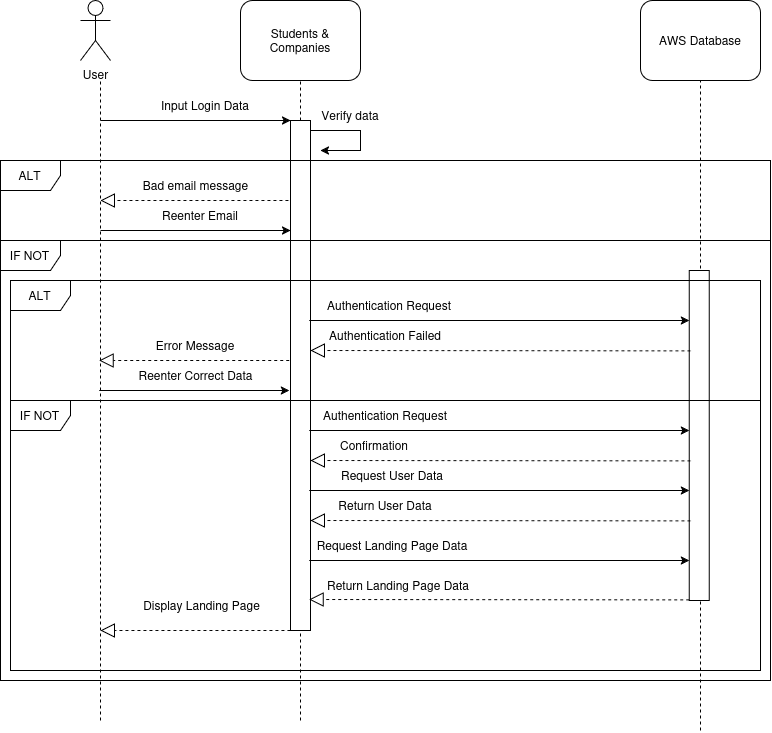
\includegraphics[width=\textwidth,height=\textheight,keepaspectratio]{RASD-Latex/assets/Use Case Diagrams/UC4.png}
    	\caption{UC4 - diagram}
    	\label{fig:DataRequest}
    \end{figure}
        
        
     \item \stepcounter{ucCounter} Edit profile \\
     \textbf{Actors:} All users\\
     \textbf{Preconditions:} The user has successfully logged into the platform and is viewing their own profile.\\
     \textbf{Success Guarantee (Postconditions):} The user successfully makes changes to their profile. \\
     \textbf{Main Success Scenario (or Basic Flow):} 
     \begin{enumerate}[label=\arabic*.] 
        \item The user presses the 'Edit' button.
        \item The platform redirects the user to the profile editing page.
        \item The user makes a change within their profile.
        \item The user presses the 'Save changes' button.
        \item The user is redirected back to viewing their profile and is informed that the changes have been saved.
     \end{enumerate} \\

    \textbf{Extensions (or Alternative Flows):} 
    \begin{enumerate}[label=\arabic*.]
        \item[*a.] At any point, the user disconnects or the system fails:
            \begin{enumerate}[label=\arabic*.]
                \item The user reconnects to the platform.
                    \begin{enumerate}[label=\alph*.]
                        \item[1a.] The platform fails to recover, or the user is unable to reconnect.
                    \end{enumerate}
                 \item The user is automatically logged back in.
                 \item The user continues from the last saved checkpoint.
            \end{enumerate}
        \item[3a.] The user makes an invalid change to their profile:
            \begin{enumerate}[label=\arabic*.]
                \item The platform informs the user that the change is not possible.
                \item The user corrects their action and proceeds with making changes.
            \end{enumerate}
        \item[1a.; 4a.] The platform is unable to redirect the user.
        \item[4a.] The changes are unable to be saved due to a server error.
        \end{enumerate}
\end{itemize}

     \begin{figure}[H]
    	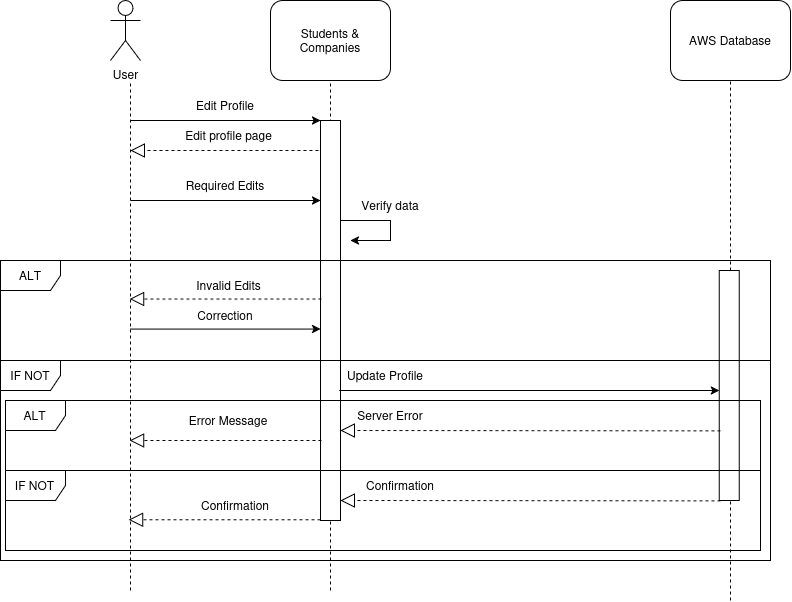
\includegraphics[width=\textwidth,height=\textheight,keepaspectratio]{RASD-Latex/assets/Use Case Diagrams/UC5.png}
    	\caption{UC5 - diagram}
    	\label{fig:DataRequest}
    \end{figure}

\newpage
\paragraph{Internship Advertisement Creation and Editing}
\begin{itemize}[label={[\textbf{UC\arabic{ucCounter}}]}, align=left, leftmargin=*]
     \item \stepcounter{ucCounter} Create and Publish Internship Advertisement \\
     \textbf{Actors:} Company Users\\
     \textbf{Preconditions:} The company user has successfully logged into the platform and is viewing the landing page. The company user has been externally verified by an admin. The company user has not reached the maximum number of advertisements.\\
     \textbf{Success Guarantee (Postconditions):} The company user successfully published an Internship Advertisement. \\
     \textbf{Main Success Scenario (or Basic Flow):} 
     \begin{enumerate}[label=\arabic*.] 
        \item The company user presses the large '+' button for creating a new advertisement. 
        \item The platform redirects the user to the advertisement creation page.
        \item The company user enters the mandatory information required for advertisement creation.
        \item The company user presses the 'Publish button'.
        \item The company user is redirected to the landing page and informed that the advertisement has been published. The company user can see his newly published advertisement.
     \end{enumerate} \\

    \textbf{Extensions (or Alternative Flows):} 
    \begin{enumerate}[label=\arabic*.]
        \item[*a.] At any point, the user disconnects or the system fails:
            \begin{enumerate}[label=\arabic*.]
                \item The user reconnects to the platform.
                    \begin{enumerate}[label=\alph*.]
                        \item[1a.] The platform fails to recover, or the user is unable to reconnect.
                    \end{enumerate}
                 \item The user is automatically logged back in.
                 \item The user continues from the last saved checkpoint.
            \end{enumerate}
        
        \item[3a.] The company user enters invalid information in the advertisement:
            \begin{enumerate}[label=\arabic*.]
                \item The platform informs the company user that the change is not possible.
                \item The user corrects their action and proceeds with advertisement creation.
            \end{enumerate}
        \item[2a.; 5a.] The platform is unable to redirect the user.
        \item[4a.] The advertisement is unable to be published due to server error.
        \end{enumerate}

     \begin{figure}[H]
    	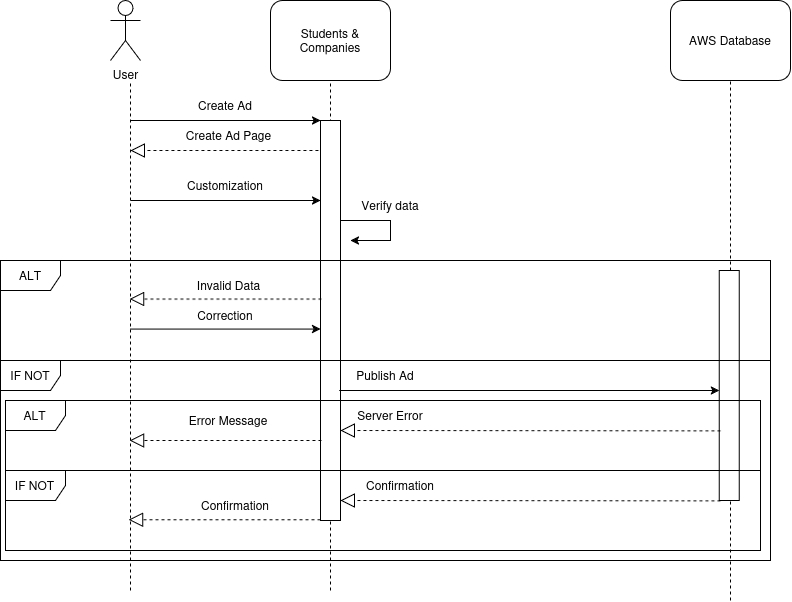
\includegraphics[width=\textwidth,height=\textheight,keepaspectratio]{RASD-Latex/assets/Use Case Diagrams/UC6.png}
    	\caption{UC6 - diagram}
    	\label{fig:DataRequest}
    \end{figure}

     \item \stepcounter{ucCounter} Edit Internship Advertisement \\
     \textbf{Actors:} Company Users\\
     \textbf{Preconditions:} The company user has successfully logged into the platform and is viewing the landing page. The company user has at least one active advertisement.\\
     \textbf{Success Guarantee (Postconditions):} The company user successfully edits an Internship Advertisement. \\
     \textbf{Main Success Scenario (or Basic Flow):} 
     \begin{enumerate}[label=\arabic*.] 
        \item The company user presses the large 'Edit' button for next to an existing internship advertisement. 
        \item The platform redirects the company user to the editing page.
        \item The company user edits the desired information required for advertisement creation.
        \item The company user presses the 'Save \& Publish button'.
        \item The company user is redirected to the landing page and informed that the advertisement edits have been made. The company user can see his newly edited advertisement.
     \end{enumerate} \\

    \textbf{Extensions (or Alternative Flows):} 
    \begin{enumerate}[label=\arabic*.]
        \item[*a.] At any point, the user disconnects or the system fails:
            \begin{enumerate}[label=\arabic*.]
                \item The user reconnects to the platform.
                    \begin{enumerate}[label=\alph*.]
                        \item[1a.] The platform fails to recover, or the user is unable to reconnect.
                    \end{enumerate}
                 \item The user is automatically logged back in.
                 \item The user continues from the last saved checkpoint.
            \end{enumerate}
        
        \item[3a.] The company user enters invalid information in the advertisement:
            \begin{enumerate}[label=\arabic*.]
                \item The platform informs the company user that the change is not possible.
                \item The user corrects their action and proceeds with advertisement creation.
            \end{enumerate}
        \item[1a.; 5a.] The platform is unable to redirect the user.
        \item[4a.] The advertisement is unable to be published due to server error.
        \end{enumerate}

     \begin{figure}[H]
    	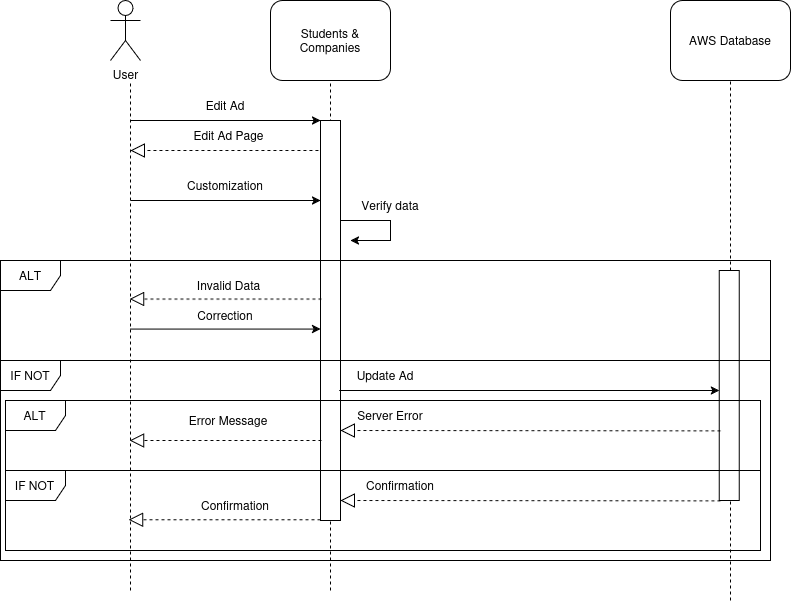
\includegraphics[width=\textwidth,height=\textheight,keepaspectratio]{RASD-Latex/assets/Use Case Diagrams/UC7.png}
    	\caption{UC7 - diagram}
    	\label{fig:DataRequest}
    \end{figure}

     \newpage
     \item \stepcounter{ucCounter} Delete Internship Advertisement \\
     \textbf{Actors:} Company Users\\
     \textbf{Preconditions:} The company user has successfully logged into the platform and is viewing the landing page. The company user has at least one active advertisement.\\
     \textbf{Success Guarantee (Postconditions):} The company user successfully deletes an Internship Advertisement. \\
     \textbf{Main Success Scenario (or Basic Flow):} 
     \begin{enumerate}[label=\arabic*.] 
        \item The company user presses the large 'Delete' button for next to an existing internship advertisement. 
        \item The system prompts the company user to check if they are certain about deletion. 
        \item The company user confirms the deletion.
        \item The company user is informed that the deletion has been made. 
     \end{enumerate} \\

    \textbf{Extensions (or Alternative Flows):} 
    \begin{enumerate}[label=\arabic*.]
        \item[*a.] At any point, the user disconnects or the system fails:
            \begin{enumerate}[label=\arabic*.]
                \item The user reconnects to the platform.
                    \begin{enumerate}[label=\alph*.]
                        \item[1a.] The platform fails to recover, or the user is unable to reconnect.
                    \end{enumerate}
                 \item The user is automatically logged back in and returned to the lading page.
            \end{enumerate}
        \item[2a.] The platform fails to display the confirmation prompt.
        \item[3a.] The advertisement is unable to be deleted due to server error.
        \end{enumerate}
     
\end{itemize}

     \begin{figure}[H]
    	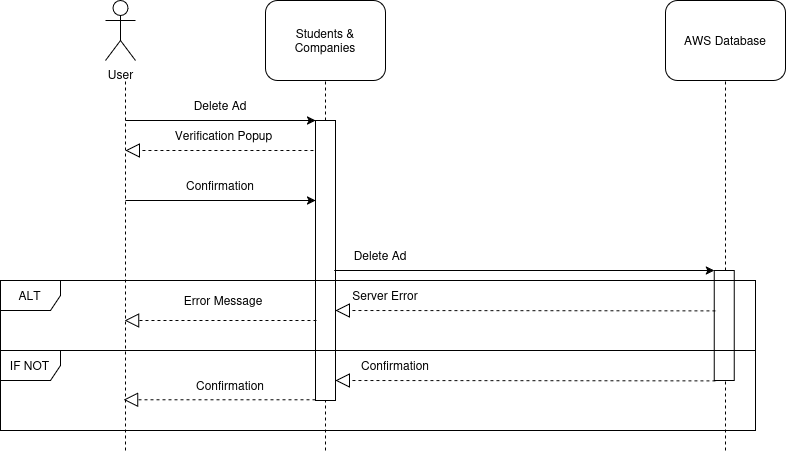
\includegraphics[width=\textwidth,height=\textheight,keepaspectratio]{RASD-Latex/assets/Use Case Diagrams/UC8.png}
    	\caption{UC8 - diagram}
    	\label{fig:DataRequest}
    \end{figure}

\paragraph{Application process}

\begin{itemize}[label={[\textbf{UC\arabic{ucCounter}}]}, align=left, leftmargin=*]
    \item \stepcounter{ucCounter} View Recommendations \& Offerings, Apply for Internship \\
     \textbf{Actors:} Student users\\
     \textbf{Preconditions:} The student user is logged into the platform and is viewing the landing page. There is at least one active internship advertisement.\\
     \textbf{Success Guarantee (Postconditions):} The student user has successfully applied for an internship. \\
     \textbf{Main Success Scenario (or Basic Flow):} 
     \begin{enumerate}[label=\arabic*.] 
        \item The student user views the available and recommended internship offerings and chooses one.
        \item The student user presses the desired advertisement 
        \item The platform redirects the user to the detailed view.
        \item The student user presses the 'Apply' button.
        \item The system produces a prompt asking the user what do they want to submit with their application.
        \item The user makes the desired selection.
        \item The user and presses 'Send'.
        \item The user is informed that the application was successful.
     \end{enumerate} \\

    \textbf{Extensions (or Alternative Flows):} 
    \begin{enumerate}[label=\arabic*.]
        \item[*a.] At any point, the user disconnects or the system fails:
            \begin{enumerate}[label=\arabic*.]
                \item The user reconnects to the platform.
                    \begin{enumerate}[label=\alph*.]
                        \item[1a.] The platform fails to recover, or the user is unable to reconnect.
                    \end{enumerate}
                 \item The user is automatically logged back in and returned to the lading page.
            \end{enumerate}
        \item[1a.] The advertisement are unable to be viewed due to server error. 
        \item[2a.] The platform is unable to redirect the user.
        \item[5a.] The platform fails to display the confirmation prompt.
        \item[4a.] The maximum number of applicants has been reached
        \end{enumerate}

        
     \begin{figure}[H]
    	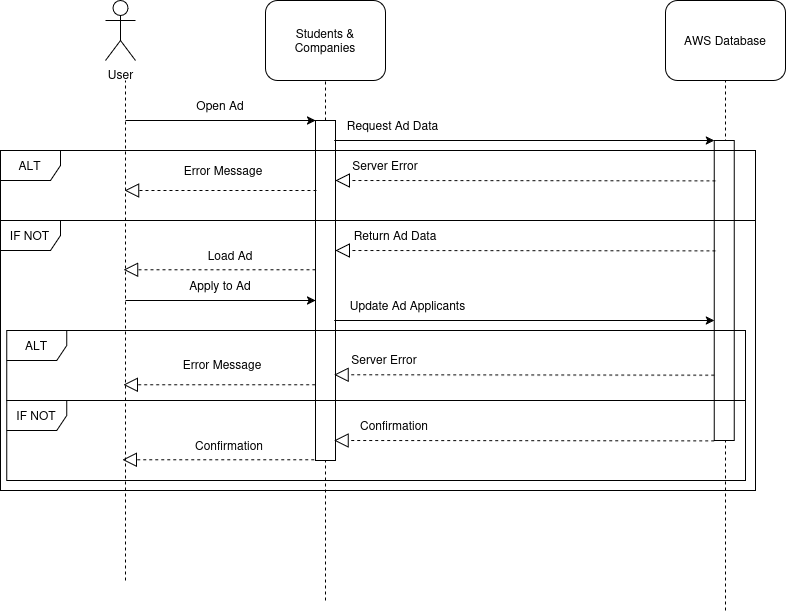
\includegraphics[width=\textwidth,height=\textheight,keepaspectratio]{RASD-Latex/assets/Use Case Diagrams/UC9.png}
    	\caption{UC9 - diagram}
    	\label{fig:DataRequest}
    \end{figure}
     
    \item \stepcounter{ucCounter} Change candidate status (increment or reject) \\
    \textbf{Actors:} Company users, Student users\\
     \textbf{Preconditions:} The company user is logged into the platform and is viewing the landing page. There is at least one active internship advertisement with at least one applicant.\\
     \textbf{Success Guarantee (Postconditions):} The company user has changed a candidates status. \\
     \textbf{Main Success Scenario (or Basic Flow):} 
     \begin{enumerate}[label=\arabic*.] 
        \item The company user selects the 'View candidates' button for the desired internship advertisement.
        \item The platform redirects the company user to the page with the list of candidates.
        \item The company user clicks the profile of a candidate they find interesting. 
        \item The platform redirects the company user to the selected candidate's profile.
        \item The company user decides to reject the candidate or move him forward in the selection process using either the 'Reject' or 'Move forward' buttons.
        \item The company user is notified that their action was successful.
        \item The selected candidate is notified via push notification that their status has changed.
     \end{enumerate} \\

    \textbf{Extensions (or Alternative Flows):} 
    \begin{enumerate}[label=\arabic*.]
        \item[*a.] At any point, the company user disconnects or the system fails:
            \begin{enumerate}[label=\arabic*.]
                \item The user reconnects to the platform.
                    \begin{enumerate}[label=\alph*.]
                        \item[1a.] The platform fails to recover, or the user is unable to reconnect.
                    \end{enumerate}
                 \item The user is automatically logged back in and returned to the lading page.
            \end{enumerate}
        \item[1a.] The advertisement are unable to be viewed due to server error. 
        \item[3a.] The candidate profile is unable to be viewed due to server error. 
        \item[2a.; 4b.] The platform is unable to redirect the user.
        \item[5a.] The platform fails to make the status change due to server error.
        \end{enumerate}

    
     \begin{figure}[H]
    	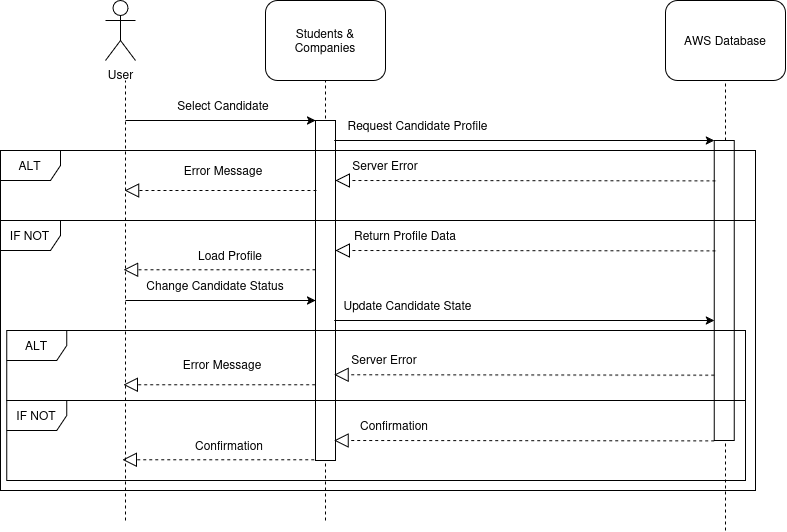
\includegraphics[width=\textwidth,height=\textheight,keepaspectratio]{RASD-Latex/assets/Use Case Diagrams/UC10.png}
    	\caption{UC10 - diagram}
    	\label{fig:DataRequest}
    \end{figure}
    
    \item \stepcounter{ucCounter} Send Prompt to Candidate (questionnaire or interview invitation)
    \textbf{Actors:} Company users, Student users\\
     \textbf{Preconditions:} The company user is logged into the platform and is viewing candidate management page for an active internship advertisement. There is at least one applicant above Stage 1.\\
     \textbf{Success Guarantee (Postconditions):} The company has successfully sent the desired prompt to the candidate. \\
     \textbf{Main Success Scenario (or Basic Flow):} 
     \begin{enumerate}[label=\arabic*.] 
        \item The company user selects the desired user and presses the 'Invite to more' button.
        \item The system provides a prompt to the company user.
        \item The company user selects whether they want an interview or if they prefer to send a questionnaire, providing additional relevant information.
        \item The company user presses the 'Send Invitation button'.
        \item The system notifies the company user that the invitation has been successful.
        \item The student user is notified about the invitation.
     \end{enumerate} \\

    \textbf{Extensions (or Alternative Flows):} 
    \begin{enumerate}[label=\arabic*.]
        \item[*a.] At any point, the company user disconnects or the system fails:
            \begin{enumerate}[label=\arabic*.]
                \item The user reconnects to the platform.
                    \begin{enumerate}[label=\alph*.]
                        \item[1a.] The platform fails to recover, or the user is unable to reconnect.
                    \end{enumerate}
                 \item The user is automatically logged back in and returned to the candidate management page.
            \end{enumerate}
        \item[1a.] The candidate profiles are unable to be viewed due to server error. 
        \item[4a.] The system fails to process the invitation due to server error.
        \end{enumerate}

    
     \begin{figure}[H]
    	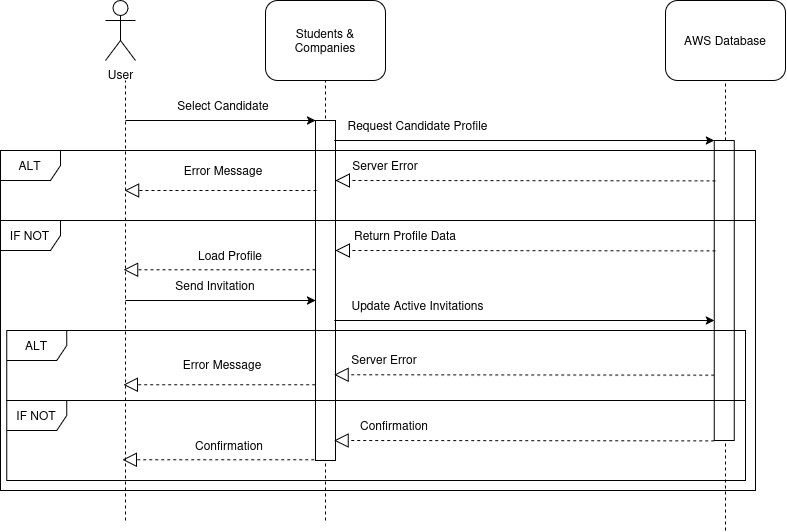
\includegraphics[width=\textwidth,height=\textheight,keepaspectratio]{RASD-Latex/assets/Use Case Diagrams/UC11.png}
    	\caption{UC11 - diagram}
    	\label{fig:DataRequest}
    \end{figure}


    \item \stepcounter{ucCounter} Reply to invitation \\
    \textbf{Actors:} Student users, Company Users\\
     \textbf{Preconditions:} The student user is logged into the platform and is viewing the landing page. The student has received an invitation.\\
     \textbf{Success Guarantee (Postconditions):} The student user has successfully replied to the invitation. \\
     \textbf{Main Success Scenario (or Basic Flow):} 
     \begin{enumerate}[label=\arabic*.] 
        \item The student user presses the 'Notifications' icon.
        \item The platform displays all notifications via a pop-up.
        \item The student views the notification and either presses the 'Reject' or 'Accept' buttons.
        \item The platform informs the student that his action was successful.
        \item The inviting company user receives a push notification about the candidate's decision.
     \end{enumerate} \\

    \textbf{Extensions (or Alternative Flows):} 
    \begin{enumerate}[label=\arabic*.]
        \item[*a.] At any point, the company user disconnects or the system fails:
            \begin{enumerate}[label=\arabic*.]
                \item The user reconnects to the platform.
                    \begin{enumerate}[label=\alph*.]
                        \item[1a.] The platform fails to recover, or the user is unable to reconnect.
                    \end{enumerate}
                 \item The user is automatically logged back in and returned to the landing page.
            \end{enumerate}
        \item[1a.] The notifications are unable to be viewed to be viewed due to server error.
        \item[4-5a.] The system is unable to process the reply due to a server error. 
        \end{enumerate}

    
     \begin{figure}[H]
    	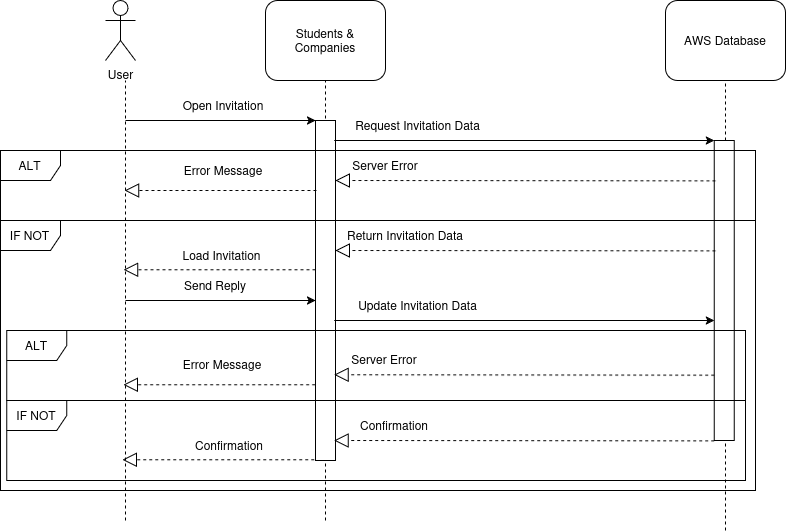
\includegraphics[width=\textwidth,height=\textheight,keepaspectratio]{RASD-Latex/assets/Use Case Diagrams/UC12.png}
    	\caption{UC12 - diagram}
    	\label{fig:DataRequest}
    \end{figure}
    
        
    \item \stepcounter{ucCounter} Initiate Internship \\
    \textbf{Actors:} Company users, University users, Student users\\
     \textbf{Preconditions:} The student user is logged into the platform and is viewing the an active internship advertisement. The company has at least one candidate who has reached the final stage.\\
     \textbf{Success Guarantee (Postconditions):} The internship has successfully been started. \\
     \textbf{Main Success Scenario (or Basic Flow):} 
     \begin{enumerate}[label=\arabic*.] 
        \item The company users views the available candidates, and selects one to begin the internship by pressing the 'Begin' button.
        \item The system notifies the relevant University user that an internship start request has been opened.
        \item The company user accepts the internship request by pressing 'Approve'.
        \item The system notifies the company user and the candidate that the internship has been initiated.
     \end{enumerate} \\

    \textbf{Extensions (or Alternative Flows):} 
    \begin{enumerate}[label=\arabic*.]
        \item[*a.] At any point, the company user disconnects or the system fails:
            \begin{enumerate}[label=\arabic*.]
                \item The user reconnects to the platform.
                    \begin{enumerate}[label=\alph*.]
                        \item[1a.] The platform fails to recover, or the user is unable to reconnect.
                    \end{enumerate}
                 \item The user is automatically logged back in and returned to the landing page.
            \end{enumerate}
        \item[1a.] The candidates are unable to be viewed to be viewed due to server error.
        \item[1b.] The request is unable to be processed due to server error.
        \item[3a.] The system is unable to process the reply due to a server error. 
        \item[3b.] The university presses the 'Reject' button.
        \begin{enumerate}[label=\arabic*.]
                \item The system notifies the company user and the candidate that the internship has been rejected by the university.
            \end{enumerate}
        
        \end{enumerate}

        
     \begin{figure}[H]
    	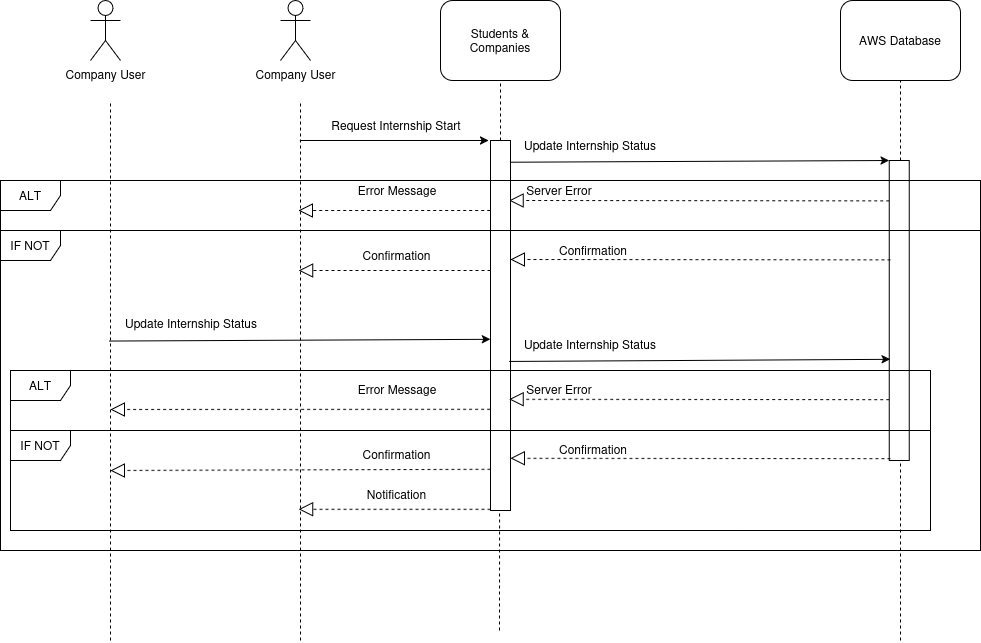
\includegraphics[width=\textwidth,height=\textheight,keepaspectratio]{RASD-Latex/assets/Use Case Diagrams/UC13.png}
    	\caption{UC13 - diagram}
    	\label{fig:DataRequest}
    \end{figure}

    \newpage
    \item \stepcounter{ucCounter} Submit Complaint \\
    \textbf{Actors:} Student users, University users\\
     \textbf{Preconditions:} The user is logged into the platform and is viewing an initiated internship.\\
     \textbf{Success Guarantee (Postconditions):} The complaint has been submitted. \\
     \textbf{Main Success Scenario (or Basic Flow):} 
     \begin{enumerate}[label=\arabic*.] 
        \item The user selects the 'Submit a complaint button' button.
        \item The platform creates a dialog box.
        \item The user enters a description of the complaint.
        \item The user presses the 'Send' button.
        \item The platform informs the user that the complaint has been sent.
        \item The relevant University is notified of the complaint.
     \end{enumerate} \\

    \textbf{Extensions (or Alternative Flows):} 
    \begin{enumerate}[label=\arabic*.]
        \item[*a.] At any point, the company user disconnects or the system fails:
            \begin{enumerate}[label=\arabic*.]
                \item The user reconnects to the platform.
                    \begin{enumerate}[label=\alph*.]
                        \item[1a.] The platform fails to recover, or the user is unable to reconnect.
                    \end{enumerate}
                 \item The user is automatically logged back in and returned to the landing page.
            \end{enumerate} 
        \item[4a.] The system fails to process the request due to server error.
        \end{enumerate}

    
     \begin{figure}[H]
    	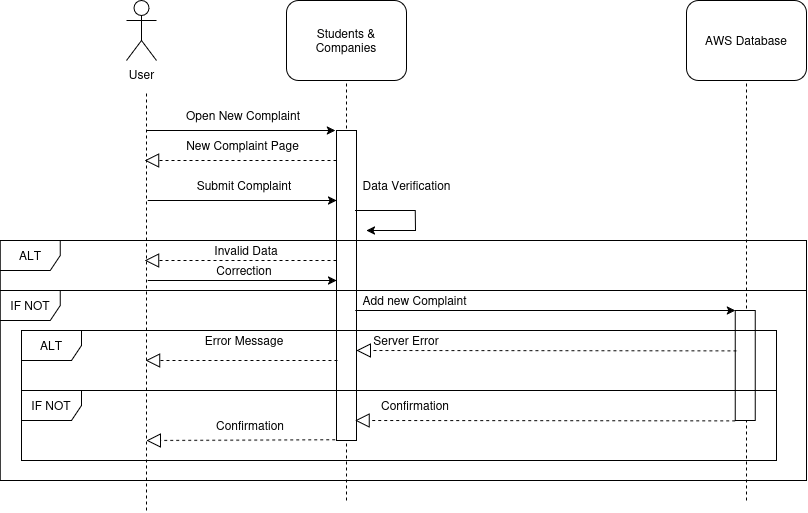
\includegraphics[width=\textwidth,height=\textheight,keepaspectratio]{RASD-Latex/assets/Use Case Diagrams/UC14.png}
    	\caption{UC14 - diagram}
    	\label{fig:DataRequest}
    \end{figure}


    \item \stepcounter{ucCounter} Resolve complaint \\
    \textbf{Actors:} Student users, Company users, University users\\
     \textbf{Preconditions:} The university user is logged into the platform and is viewing the list of active complaints.\\
     \textbf{Success Guarantee (Postconditions):} The submitted complain has successfully been resolved. \\
     \textbf{Main Success Scenario (or Basic Flow):} 
     \begin{enumerate}[label=\arabic*.] 
        \item The university user views the list of complaints, and selects the complaint they wish to work on.
        \item The platform displays a preview of the complaint, with an open input field.
        \item The university user fills the field with the reply.
        \item The university user presses the 'Submit reply \& Close'.
        \item The platform informs the university user that the change was successful.
        \item The relevant Company user and Student users are are notified of the complaint's resolution.
     \end{enumerate} \\

    \textbf{Extensions (or Alternative Flows):} 
    \begin{enumerate}[label=\arabic*.]
        \item[*a.] At any point, the company user disconnects or the system fails:
            \begin{enumerate}[label=\arabic*.]
                \item The user reconnects to the platform.
                    \begin{enumerate}[label=\alph*.]
                        \item[1a.] The platform fails to recover, or the user is unable to reconnect.
                    \end{enumerate}
                 \item The user is automatically logged back in and returned to the landing page.
            \end{enumerate} 
        \item[4a.] The system fails to process the request due to server error.
        \end{enumerate}

\end{itemize}


     \begin{figure}[H]
    	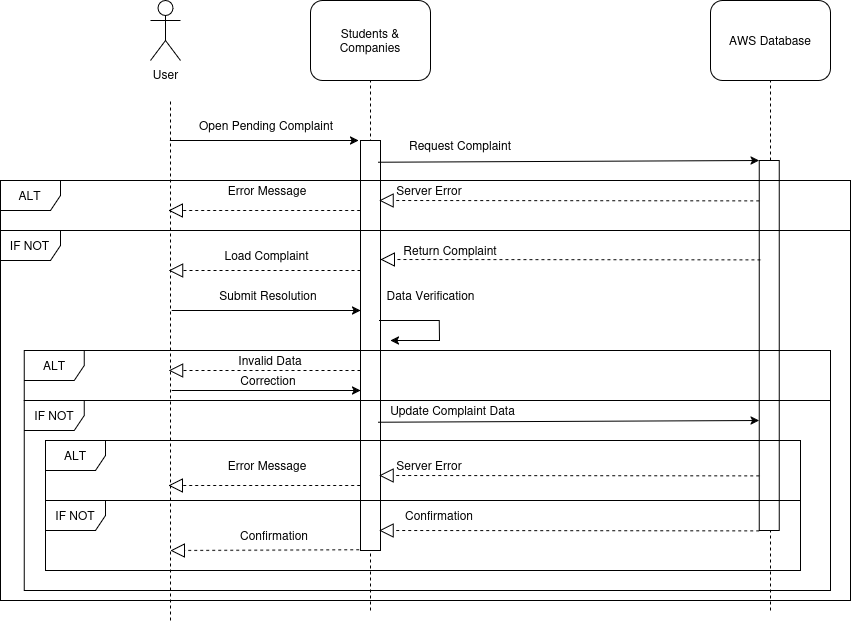
\includegraphics[width=\textwidth,height=\textheight,keepaspectratio]{RASD-Latex/assets/Use Case Diagrams/UC15.png}
    	\caption{UC15 - diagram}
    	\label{fig:DataRequest}
    \end{figure}


\paragraph{Feedback management}

\begin{itemize}[label={[\textbf{UC\arabic{ucCounter}}]}, align=left, leftmargin=*]
    \item \stepcounter{ucCounter} Submit feedback. \\
    \textbf{Actors:} Student users, Company users, University users\\
     \textbf{Preconditions:} An internship has been successfully finished. The user is notified of a pending internship review.\\
     \textbf{Success Guarantee (Postconditions):} The feedback has been successfully submitted. \\
     \textbf{Main Success Scenario (or Basic Flow):} 
     \begin{enumerate}[label=\arabic*.] 
        \item The user presses the 'Notifications' icon.
        \item The platform displays all notifications via a pop-up.
        \item The student views the pending review notification and clicks on it.
        \item The platform redirects the user to a predetermined form.
        \item The user enters the relevant data.
        \item The user presses the 'Submit button'.
        \item The platform informs the user that his action was successful.
        \item The other relevant users get notified of the submitted feedback.
     \end{enumerate} \\

    \textbf{Extensions (or Alternative Flows):} 
    \begin{enumerate}[label=\arabic*.]
        \item[*a.] At any point, the company user disconnects or the system fails:
            \begin{enumerate}[label=\arabic*.]
                \item The user reconnects to the platform.
                    \begin{enumerate}[label=\alph*.]
                        \item[1a.] The platform fails to recover, or the user is unable to reconnect.
                    \end{enumerate}
                 \item The user is automatically logged back in and returned to the landing page.
            \end{enumerate}
        \item[1a.] The notifications are unable to be viewed to be viewed due to server error.
        \item[6a.] The system is unable to process the reply due to a server error. 
        \end{enumerate}

        
     \begin{figure}[H]
    	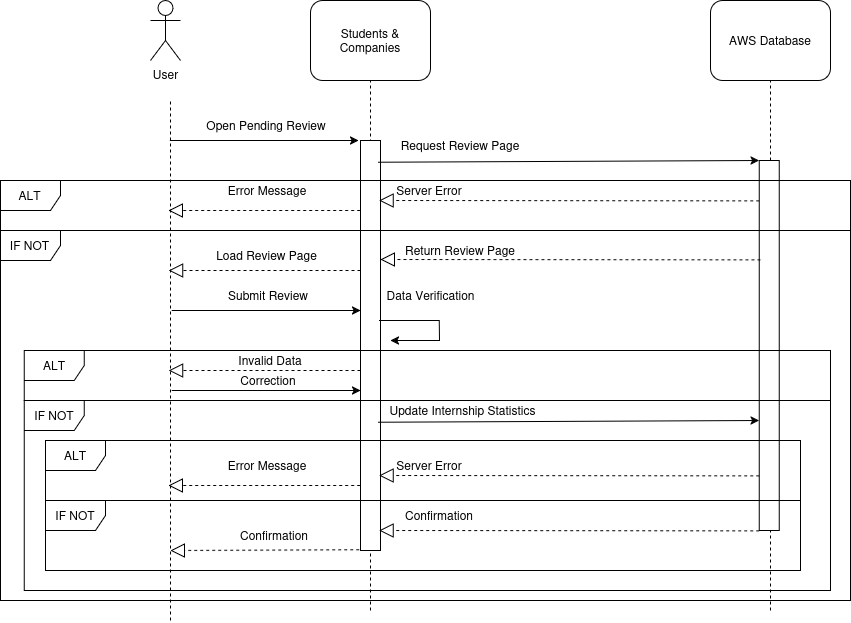
\includegraphics[width=\textwidth,height=\textheight,keepaspectratio]{RASD-Latex/assets/Use Case Diagrams/UC16.png}
    	\caption{UC16 - diagram}
    	\label{fig:DataRequest}
    \end{figure}


    \item \stepcounter{ucCounter} View feedback. \\
    \textbf{Actors:} Student users, Company users, University users\\
     \textbf{Preconditions:} An internship has been successfully finished. All feedback has been submitted.\\
     \textbf{Success Guarantee (Postconditions):} The feedback has been viewed. \\
     \textbf{Main Success Scenario (or Basic Flow):} 
     \begin{enumerate}[label=\arabic*.] 
        \item The user presses the 'Notifications' icon.
        \item The platform displays all notifications via a pop-up.
        \item The student views the new feedback notification and clicks on it.
        \item The platform displays the feedback to the user regarding that particular internship.
     \end{enumerate} \\

    \textbf{Extensions (or Alternative Flows):} 
    \begin{enumerate}[label=\arabic*.]
        \item[*a.] At any point, the company user disconnects or the system fails:
            \begin{enumerate}[label=\arabic*.]
                \item The user reconnects to the platform.
                    \begin{enumerate}[label=\alph*.]
                        \item[1a.] The platform fails to recover, or the user is unable to reconnect.
                    \end{enumerate}
                 \item The user is automatically logged back in and returned to the landing page.
            \end{enumerate}
        \item[1a.] The notifications are unable to be viewed to be viewed due to server error.
        \end{enumerate}
\end{itemize}


     \begin{figure}[H]
    	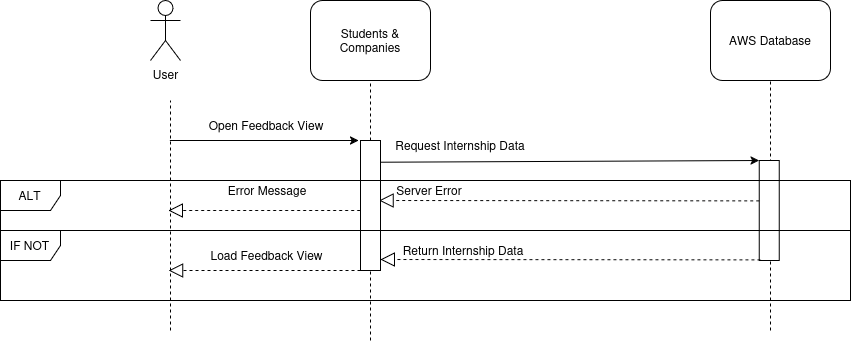
\includegraphics[width=\textwidth,height=\textheight,keepaspectratio]{RASD-Latex/assets/Use Case Diagrams/UC17.png}
    	\caption{UC17 - diagram}
    	\label{fig:DataRequest}
    \end{figure}



\subsubsection{Sequence diagrams}
\subsubsection{Requirement mapping}
The following section assesses each goal as listed in section 1.1.1, and presents which Domain Assumptions (D) and Functional Requirements(FR) match them. In cases 

\begin{enumerate}[label={\textbf{[G\arabic*]}}]
    \item \textbf{Companies create internship advertisement.} 
    \begin{enumerate}[label={\textbf{[D\arabic*]}}]
        \item[\textbf{[D4]}] Companies provide accurate information about an internship.
        \item[\textbf{[D7]}] Companies respond to applications promptly.
    \end{enumerate}
    \begin{enumerate}[label={\textbf{[D\arabic*]}}]
        \item[\textbf{[FR10-FR15]}] Cover the registration of company users.
        \item[\textbf{[FR20-FR25]}] Cover the creation, update, and management of internship advertisements.
    \end{enumerate}
    
    \item \textbf{Students find appropriate internship and initiate contact with the selected company.}
    \begin{enumerate}[label={\textbf{[D\arabic*]}}]
        \item[\textbf{[D1]}] User must have a reliable internet connection.
        \item[\textbf{[D2]}] All users provide accurate information when creating profiles.
        \item[\textbf{[D7]}] Companies respond to applications promptly.
        \item[\textbf{[D8]}] Students complete selection process steps within deadlines.
    \end{enumerate}
    \begin{enumerate}[label={\textbf{[D\arabic*]}}]
        \item[\textbf{[FR1-FR3]}] Cover registration and login for student users.
        \item[\textbf{[FR16-FR18]}] Cover profile management by students.
        \item[\textbf{[FR26-FR29]}] Cover searching, applying, and notification about internships.
    \end{enumerate}
    
    \item \textbf{Students become interns in the companies in order to gain experience in the desired area of industry.}
    \begin{enumerate}[label={\textbf{[D\arabic*]}}]
        \item[\textbf{[D2]}] All users provide accurate information when creating profiles.
        \item[\textbf{[D4]}] Companies provide accurate information about an internship.
        \item[\textbf{[D8]}] Students complete selection process steps within deadlines.
    \end{enumerate}
    \begin{enumerate}[label={\textbf{[D\arabic*]}}]
        \item[\textbf{[FR28-FR30]}] Cover internship application and selection process..
        \item[\textbf{[FR32]}] Cover initiation of internships by companies and universities.
    \end{enumerate}
    
    \item \textbf{The platform provides a transparent and fair selection process where companies can evaluate and select suitable candidates.}
    \begin{enumerate}[label={\textbf{[D\arabic*]}}]
        \item[\textbf{[D7]}] Companies respond to applications promptly.
        \item[\textbf{[D8]}] Students complete selection process steps within deadlines.
    \end{enumerate}
    \begin{enumerate}[label={\textbf{[D\arabic*]}}]
        \item[\textbf{[FR29-FR31]}] Cover movement of candidates through stages, rejection, and acceptance notifications.
        \item[\textbf{[FR32]}] Cover approval of internships by universities.
    \end{enumerate}
    
    \item \textbf{The platform offers a recommendation system that matches students to internships based on their CVs, skills, and preferences, as well as company requirements.}
    \begin{enumerate}[label={\textbf{[D\arabic*]}}]
        \item[\textbf{[D2]}] All users provide accurate information when creating profiles.
    \end{enumerate}
    \begin{enumerate}[label={\textbf{[D\arabic*]}}]
         \item[\textbf{[FR26]}] Cover the recommendation system for internships based on student profiles.
    \end{enumerate}
    
    \item \textbf{The platform allows universities to monitor internships to ensure alignment with academic standards.}
    \begin{enumerate}[label={\textbf{[D\arabic*]}}]
        \item[\textbf{[D3]}] Universities actively engage with the platform in order to monitor active internships and to resolve complaints.
    \end{enumerate}
    \begin{enumerate}[label={\textbf{[D\arabic*]}}]
         \item[\textbf{[FR33]}] Cover monitoring by universities during internships.
         \item[\textbf{[FR34, FR35]}] Cover feedback collection and review by universities.
    \end{enumerate}
    
    \item \textbf{The platform collects feedback from both students and companies to improve the platform’s functionality.}
    \begin{enumerate}[label={\textbf{[D\arabic*]}}]
        \item[\textbf{[D4]}] Companies provide accurate information about an internship.
        \item[\textbf{[D6]}] Submitted complaints are genuine and not misused to create unnecessary conflicts.
    \end{enumerate}
    \begin{enumerate}[label={\textbf{[D\arabic*]}}]
         \item[\textbf{[FR36,FR37]}] Cover feedback collection after internships.
         \item[\textbf{[FR38]}] Cover review and optional publication of feedback by universities.
    \end{enumerate}
    
    \item \textbf{Ensure a safe and supportive environment by providing students with mechanisms to file complaints and enabling universities to resolve them.}
    \begin{enumerate}[label={\textbf{[D\arabic*]}}]
        \item[\textbf{[D3]}] Universities actively engage with the platform in order to monitor active internships and to resolve complaints..
        \item[\textbf{[D6]}] Submitted complaints are genuine and not misused to create unnecessary conflicts.
    \end{enumerate}
    \begin{enumerate}[label={\textbf{[D\arabic*]}}]
         \item[\textbf{[FR33,FR34]}] Cover submission and resolution of complaints.
         \item[\textbf{[FR35]}] Cover termination of internships based on complaints.
    \end{enumerate}
    
\end{enumerate}